\section{Nebulas Rank算法}


\subsection{Introduction} \label{sec:intro}
Ranking nodes in complex network has been a fundamental concern in various applications. One canonical example is PageRank\cite{Brin2010}\cite{page1999pagerank}, which is the core algorithm for Google and other search engines\cite{langville2011google}. Besides, by ranking algorithm, people also want to find out the most influential spreaders in epidemic and information network\cite{doerr2012rumors}\cite{Kitsak2010}, the most acknowledged scientist by the citation network or co-author network\cite{walker2007ranking}\cite{chen2007finding}\cite{Radicchi2009}, the most important cities in the transportation network\cite{guimera2005worldwide}, the most important vertices in metabolic network\cite{ivan2010web}, the top VC firms by co-investment\cite{Bhat2012} etc. And when it comes to designing \textbf{Nebulas Rank} algorithm for blockchain world, decades of researches have enlightened us with many measurements like degree centrality\cite{freeman1979set}, eigenvector centrality\cite{bonacich1972factoring}, Katz centrality\cite{katz1953new}, PageRank\cite{Brin2010}, HITS\cite{kleinberg1999authoritative}, closeness centrality\cite{sabidussi1966centrality}, betweenness centrality\cite{freeman1977set}\cite{freeman1978centrality}\cite{freeman1991centrality}\cite{noh2004random}\cite{newman2005measure}, etc. Before building our algorithm on the top of them, however, we still need to answer two questions:
\begin{enumerate}
\item What properties are embedded in the network?
\item What value should the rank indicate?
\end{enumerate}
For the first question, \textbf{Nebulas Rank} uses the transaction graph of blockchain system, which is generated by the transaction history during the past period. We compare blockchain transaction graph with others in three aspects. First, as node representing accounts and edges representing money transferring, basically, the graph is a weighted directed graph, bearing large difference from social network\cite{Ugander2011} and similarity with webpage network\cite{page1999pagerank} in terms of topology. An asymmetric edge indicates the imbalanced ability of controlling money between two nodes. And edges' weight also characterizes the difference among links' quality. Thus directly applying standard algorithms for unweighted or undirected graph could discard a lot important information. Second, since the graph is derived by the trajectory of money flow, it could be presumed that Exchanges are highly ranked, whereas such accounts are willing to swap money with any client. Thus anyone can acquire unlimited links from those existing important nodes without much cost. Along with the anonymity of typical blockchain systems, sybil attackers could make large amount of transferring with a big Exchange account, in order to improve his influence such as PageRank. (It is still hard to receive money from a large number of non-sybil nodes, though.) This is an essentially difference from applications previously studied. For example, in an online social network with subscription relation, it costs no effort to follow an opinion leader, while attracting a verified opinion leader's attention is not an trivial thing. Third, being different from Bitcoin\cite{Nakamoto2008}, the newly invented blockchain systems such as Ethereum\cite{Wood2014} introduces "smart contract" as a new type of account. After a normal account invoking some method of a contract, a sequence of consequent callings will be raised forming part of a call graph. Unlike Bitcoin transaction graph, which only contains money transferring, Ethereum call graph/network also represents dynamic programming calling. We believe such network embeds more information and should be useful to measure a DApp or smart contract's value.

For the second question, \textbf{Nebulas Rank} aims to measure the value of users, and smart contracts in blockchains. For normal accounts, we define value by two aspects: \textbf{Liquidity}, which stresses the ability to control digital assets flow of high quality; \textbf{Propagation}, which focus more on the spreading influence. For smart contracts, we also consider \textbf{Interoperability} as a measurement. There are three-fold purposes in \textbf{Nebulas Rank}: 1) to be a good metric for blockchain accounts and smart contract search engine; 2) to provide a trustful criteria in PoR consensus protocol (see \refsec{}) , where only high ranked accounts should be eligible to become a validator; 3) to help to build DIP mechanism (see \refsec{}). \footnote{Note the in this section, our transaction data don't include smart contracts. More about DIP is described in \refsec{}}.

More clearly, \textbf{Nebulas Rank} should be based on the formal concept of network flow. As revealed in \cite{Borgatti2005}, most centralities can be classified by their type of network flow. From the dimension of diffusion mechanism, traffic flow can spread by different kinds of duplication or transfer. Another spectrum is the trajectory of flow, which can be either paths, trails or walks. Essentially, blockchain transaction graph is the trajectory of money exchange, which falls into the classification of "transfer walk". Imagine an amount of money enters the network. Then the owner node divides the money and transfers to neighbors or keep it. To clarify, the money is divisible, imperishable and non-replicable and each step's direction is random due to the limit of local information. This rules out some measurements for us. For example, \textcite{freeman1977set}'s betweenness centrality, since it implies geodesic optimal paths.

Following are our solutions to the challenges described above.

First, in order to turn transactions into a graph, we keep the transfer value as edges' weight and embed the transfer timestamp into nodes' coinage property. Then we exploit coinage and other properties to fix the edge weight:
\begin{itemize}
	\item We set a time window of $T$ days and aggregate the largest $K$ transactions as an edge's weight. (see \refsec{subsec:aggreate};
	\item We reduce each edge's weight by its target's "coinage". In order to get higher coinage, an owner needs to let the money stay in place for a while, which slows down the speed of sybil attacks such as loop attack. (see \refsec{subsec:coinage})
	\item Edge weight is also reduced by its target's outgoing amount(see \refsec{subsec:limit}) as well as an encouragement function (see \refsec{subsec:encouragement}), which helps to mitigate some undesired effect.
\end{itemize}

Second, with graph generated, we measure each node's importance based on Weighted LeaderRank algorithm\cite{Chen2013}\cite{Li2014}. LeaderRank is a simple variant of PageRank, which adds a ground node into the network and connect the ground node with each non-ground node. It substitutes PageRank's teleportation parameter by links throughout ground node, which is said to be more effective in computing, robust against manipulations and noise than PageRank algorithm\cite{Chen2013}. The intuition for both LeaderRank and PageRank is random walk and Markov Chain. By PageRank, from each node, the probability of jumping to an arbitrary node is the same (or equal to 1 if there is no out links \cite{Kim2002}). Whereas by LeaderRank\cite{Li2014}\cite{Chen2013}, different nodes adopt different arbitrary transition probabilities. For example, we could allow a node with more in-links to receive more teleportation probability. This is more plausible in the context of blockchain, since an account with little money transferred in is less trustable. Also, if a node receives much money but hardly spend it, we suppose it has more "surplus value" and assign with more teleportation probability from it. We will talk about the details of LeaderRank scheme in \refsec{sec:leaderrank}.

Intuitively, LeaderRank indicates the flux over a node in the dynamic equilibrium of money exchange network flow. From another perspective, mode flux means more control. The LeaderRanks algorithm matches both our goals of measuring \textbf{Liquidity} and \textbf{Propagation}. Although some other betweenness based algorithm such as flow betweenness\cite{freeman1991centrality} and random walk betweenness (aka. current flow betweenness)\cite{newman2005measure} may be more suitable to represent the flow controlling ability, these centralities are quite computational intensive. So they are not suitable for \textbf{Nebulas Rank}. Besides, there are some more thinkings during the design of \textbf{Nebulas Rank}. For example, network clustering may also be helpful to depreciate spam nodes\cite{Nikolakopoulos2013}. But it is also defective to overexploit the clustering effect. All issues will be discussed at \refsec{sec:discuss}.

\st{Our experiment results shows that ...... }

The rest of paper is organized as follows. \refsec{sec:related} introduces the related works. Then in \refsec{sec:txg}, we define the network topology and weight based on blockchain transactions. And in \refsec{sec:leaderrank}, LeaderRank with schemes designed for \textbf{Nebulas Rank} is introduced. In \refsec{sec:exp}, we show our experiment results. And Finally we give all discussions and conclusions in \refsec{sec:discuss}

\subsection{Related Works} \label{sec:related}
Centrality, the core ranking index, is a most studied concept in network science since decades ago\cite{newman2010networks}. There are a body of literatures introducing various centralities, including degree centrality\cite{freeman1979set}, eigenvector centrality\cite{bonacich1972factoring}, Katz centrality\cite{katz1953new}, closeness centrality\cite{sabidussi1966centrality}, betweenness centrality\cite{freeman1977set}\cite{freeman1978centrality}\cite{freeman1991centrality}\cite{noh2004random}\cite{newman2005measure}, PageRank\cite{Brin2010}, HITS\cite{kleinberg1999authoritative}, SALSA\cite{Science2001}, etc. It is fundamental to clearly classify these measurements by a unified framework. \textcite{Borgatti2005} adopts a network flow based view to classify the centrality measurements by two categorical dimensions: material flowing by parallel duplication, serial duplication and transfer; and trajectory following geodesics optimum, path, trail and walk. \textcite{Borgatti2006} propose a unified framework with four dimensions from the perspective of graph theory. \textcite{Lu2016} review representative centrality algorithms and classified them into those only based on structural information, those driven by Markov dynamics, those by looking at the effect of removing nodes, those with dynamics-sensitivity and those trying to identify more than one node. With a hierarchical understanding of centrality algorithms, we are able to choose appropriate strategy according to the network scenarios. \textbf{Nebulas Rank}'s scenario is the money exchange flow network mentioned in \cite{Borgatti2005}.

Since Bitcoin\cite{Nakamoto2008} system released in 2009, researchers have done some statistical and empirical analysis on Bitcoin's transaction graph\cite{Ron}\cite{Haslhofer}\cite{NielKondor2014}\cite{Baumann2014}, and some use the transaction graph structure to discuss anonymity in Bitcoin\cite{Meiklejohn2013}\cite{Ober2013}\cite{pham2016anomaly}\cite{Fleder2015}\cite{Ferrin2015}. After other cryptocurrencies emerged and become popular, transaction graph analysis is conducted with more blockchains\cite{Chang2017}\cite{Anderson2016}. \textbf{Nebulas Rank} adopts their transaction graph concept, i.e. Entity Graph in \cite{Tschorsch2015}, with minor revisions. That is, each account, or set of accounts belonging to the same people, is mapped as a node. And each directed edge represents the intensity of transferring between two accounts. Actually before blockchain system like Bitcoin was invented, scientists have tried to study some financial networks among banks and global trading entities\cite{propper2008towards}\cite{Boss2004}\cite{Serrano2007}\cite{Bech2008}\cite{Fagiolo2009}\cite{Morten2006}\cite{Boss2004a}\cite{Krempel2002}\cite{Serrano2003}. Comparing with blockchain transaction networks, these early studied finical networks are defined not only by transferring activities, but also by lending-based relationship. Moreover, the scale of these networks is much smaller. To conclude, there is rarely research work proposing custom ranking method for large scale transaction graph, especially blockchain transaction graph.

The most relevant work with \textbf{Nebulas Rank} is NEM\cite{nem}'s Proof-of-Importance scheme. It adopts NCDawareRank\cite{Nikolakopoulos2013}, which exploits the clustering effect of network topology, as the ranking algorithm, with clustering algorithm based on SCAN algorithm\cite{xu2007scan}\cite{shiokawa2015scan}\cite{chang2017mathsf}. And \textcite{Fleder2015} uses PageRank\cite{Brin2010}\cite{page1999pagerank} as an assisting metric to discover interesting addresses and analyze their activities. However, both NCDawareRank and PageRank are ranking algorithms for webpage network. As we already mentioned in \refsec{sec:intro}, blockchain transaction graph is very different from webpage network. And although community structure does exist in transaction graph and should be helpful to handle with spam nodes, it does not suit the consensus purpose mentioned in \refsec{sec:intro}. Because in order to compute "unforgeable" node importance, accounts controlled by a single "real world" entity should be guaranteed to be mapped to the same cluster. However it is key difficulty to connect blockchain world with the "real world", and thus there is no proper objective definition for clustering problem. Therefore current clustering algorithms cannot provide meaningful and trustful result. Moreover, \cite{Fleder2015}'s work does not provide an automated framework to identify important nodes. Instead, it still needs manual analyzing with the help of PageRank, which does not match \textbf{Nebulas Rank}'s context.

The algorithm we choose is LeaderRank\cite{Chen2013}\cite{Li2014}. It is a simple variant of PageRank\cite{Brin2010}\cite{page1999pagerank}. In PageRank, initially every node gets one unit rank value. Then at each iteration, every node distributes its rank value equally to its directed neighbors. To deal with dangling node problem, there is a damping factor, where every node distribute a specific proportion of its rank value to all nodes equally in the network. \textcite{Chen2013} propose a simple yet effective modification on PageRank's damping factor and call it LeaderRank. Then \textcite{Li2014} extend LeaderRank to weighted case and further improve its performance. By weighted LeaderRank\cite{Li2014}, an additional ground node is added and a bidirectional link is added between every node and ground node. Every edge targeting to ground node is of same weight and every edge from ground node is weighed positively proportional to target node's in-degree. LeaderRank is more resistant against manipulation and noisy data than PageRank\cite{Chen2013}\cite{Li2014}\cite{Lu2016}. In terms of computation, LeaderRank can be seen as PageRank with one more node and set damping factor to be zero. And thus it is easy to implement and very scalable. There are also other algorithms modifying PageRank's damping factor mechanism. For example, \textcite{Baeza-Yates2006} proposed a damping function decreasing with distance. Out of all the current algorithms, we think LeaderRank is a relatively simple and effective one. We will modify LeaderRank a little and discuss more on its weighting scheme at \refsec{sec:leaderrank}.

\subsection{Transaction Graph} \label{sec:txg}

\subsubsection{Transactions}\label{subsec:transfer}
The input data for \textbf{Nebulas Rank} are all the transaction records, i.e. token transferring, during the past $T$ days, denoted by a set of tuples:
$$
	T_{xs}^{all} = \{(s,t,\tau, a), \tau = Today-T \dots Today \}
$$
, where $s$, $t$ and $a$ are the source account, target account and amount of an transfer, respectively.

Further, we filter transactions, providing that self transfer and zero amount transfer are excluded:
\begin{align}
	T_{xs} = \{(s,t,\tau, a)| s \neq t \land a > \Phi \land (s,t,\tau, a) \in T_{xs}^{all} \}, \Phi = 0
\end{align}

\subsubsection{Transactions Aggregation} \label{subsec:aggreate}
 Based on transactions defined above, we construct the directed weighted transaction graph $G=(V, E, W)$, where node set, edge set and weight on edges are denoted by $V$, $E$ and $W$ respectively. We also denote that $N = |V|$ and $M = |E|$. For simplicity, all nodes are denoted by integer numbers from $1$ to $N$.

Each vertex $v \in V$ represents one individual account's address. Each edge represents the transferring intensity between two accounts. Consider $e=(s,t) \in E$, this edge is directed, and naturally, the weight of it should be determined by all related transactions, i.e. $(s,t,\tau, a) \in T_{xs}$. To compute edge $(s,t)$'s weight, we take the sum of top $K$ amounts out of all related transactions:
\begin{align}\label{formula:edgeweight}
w_e = \sum_{i=1}^K a_i, s.t. a_i \in \{a|(s,t,\tau,a) \in T_{xs} \} \land a_1 \geq a_2 \dots
\end{align}

By this mean, the link between two nodes is bi-directed and asymmetric, with top $K$ transactions along each direction aggregated to become the weight. This is different from NEM, which all transfers amounts between two nodes are aggregated into one unilateral edge's weight\cite{nem}. We presume NEM's solution is vulnerable to manipulations, since only a simple triangle loop will enhance edges' weight into infinity. Additionally, it is also not truthful to take the average or quartile of all relation transactions, since this forces accounts to transfer very cautiously. We will show the advantage of our aggregation method in \refsec{} \st{experiment confirming why doing so}

\subsubsection{Temporality Embedding} \label{subsec:coinage}
We noticed that the transactions happens with timestamps. So we try to embed this temporal information as a property of nodes. For each account, we calculate its coinage by the following pseudo-code.

\st{formula} \st{Defined as $C_v$ normalized by max}

\begin{figure}
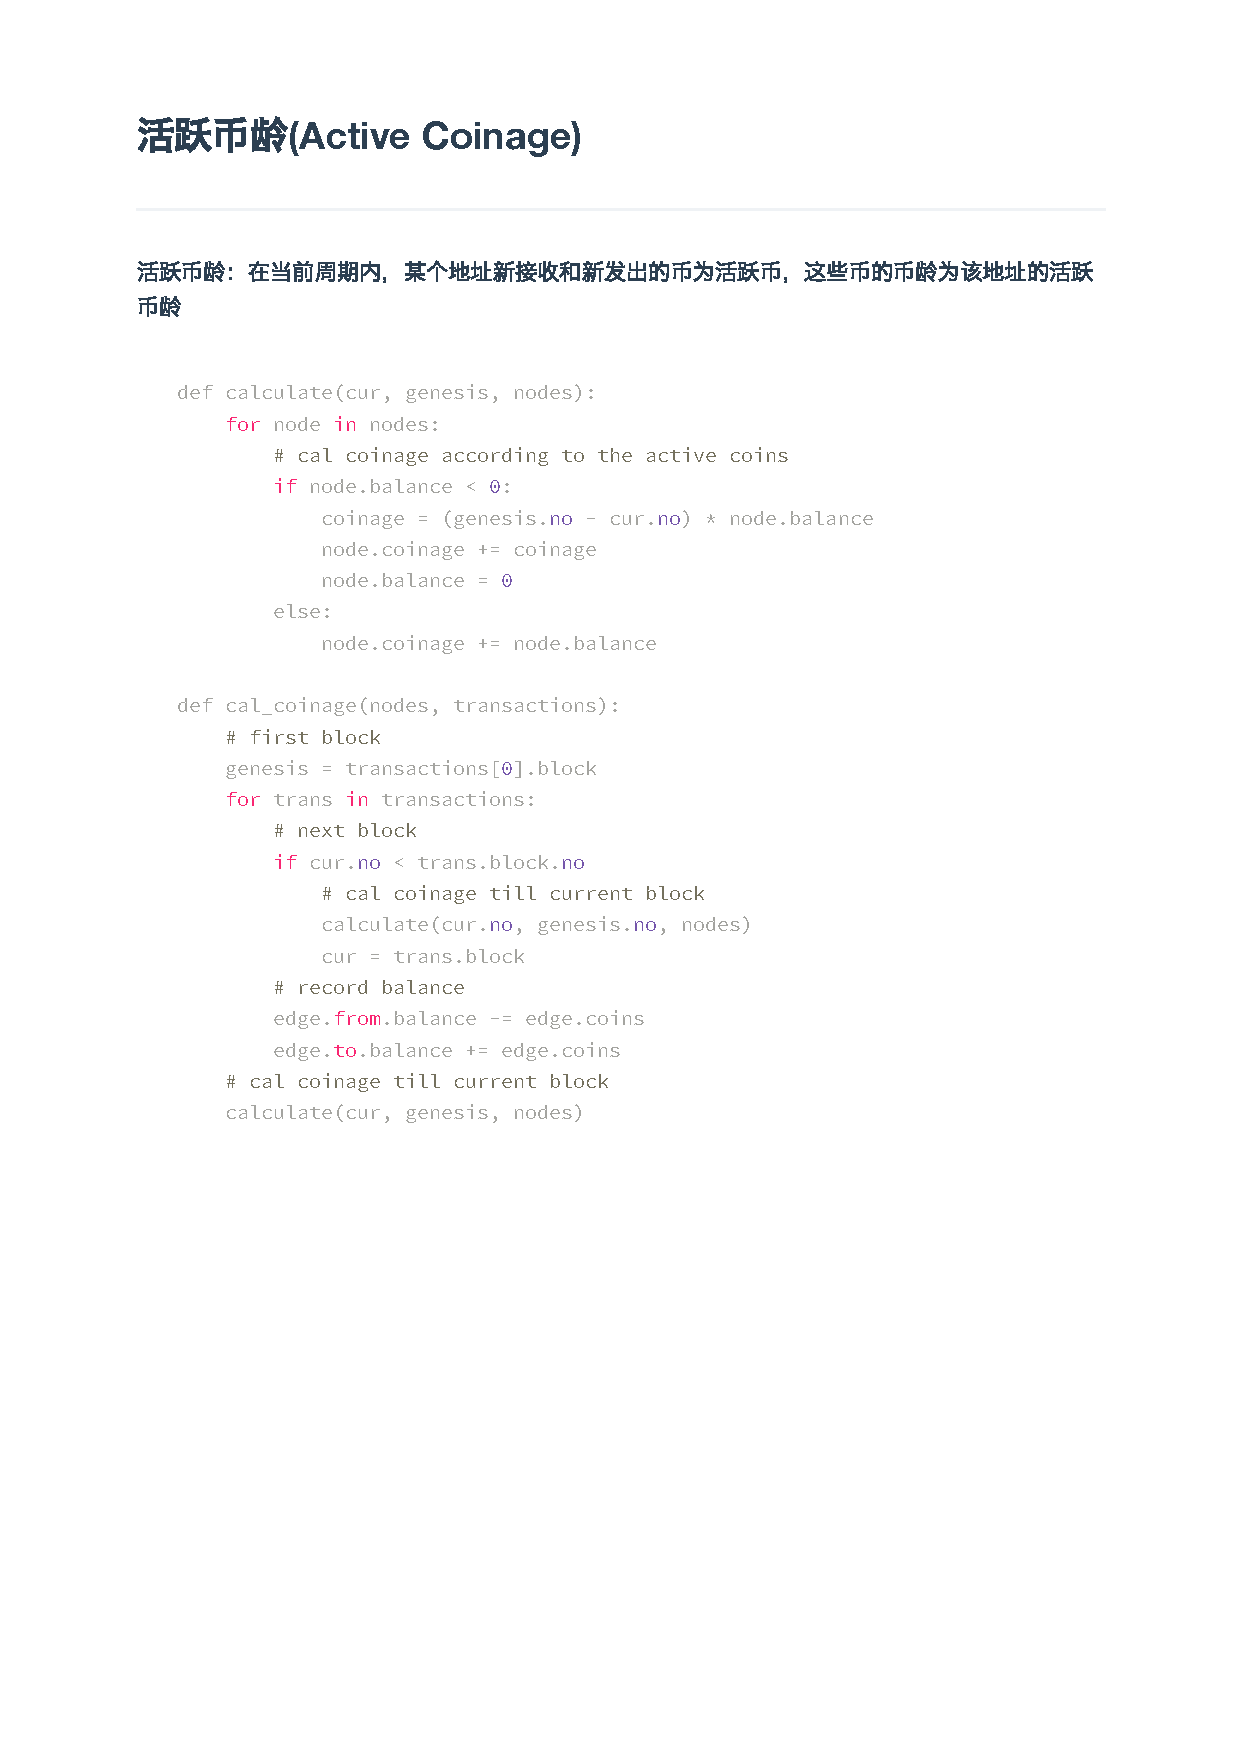
\includegraphics{coinage.pdf}
\end{figure}


The intuition of coinage is \st{insights}.

Besides, we conjecture that reducing each transaction's contribution according to its block height, like NEM does\cite{nem}, encourages users to postpone their transferring until the last day of period, which will cause unnecessary confusion. Instead, \textbf{Nebulas Rank} treats each transaction equally, which encourages every account to keep active all the time.

We will talk about the coinage exploitation in \refsec{subsec:reduction}. And we will show the advantage of our solution in \refsec{} \st{experiments confirming the effect of coinage}.


\subsubsection{Encouragement Function}\label{subsec:encouragement}
\st{formula and intuition} \st{defined as $B_v$ normalized by max}

We will talk about how we apply the encouragement function in \refsec{subsec:reduction}. And we will show its advantage in \refsec{} \st{experiments confirming the effect of encouragement function}.

\subsubsection{Exploiting Nodes' Property} \label{subsec:reduction}
We defined two node properties $C_v$ and $B_v$ in \refsec{subsec:coinage} and \refsec{subsec:encouragement}, respectively. Then we reduce each edge's weight by its target node's properties:
\begin{align}\label{formula:exploit}
	w_{(.,v)} \leftarrow w_{(.,v)} \times ln(1 + \frac{C_v + B_v}{2})
\end{align}

\subsubsection{Mitigating Dormant Effect} \label{subsec:limit}
Consider a node receiving a large amount of money but does not spend any. This node forces its money to be "dormant " and prevents money from being circulated, which contradicts with \textbf{Nebulas Rank}'s purpose(\refsec{sec:intro}). Thus we need to mitigate this dormant effect. In detail, we consider 1-hop local information of each node, limiting the amount of its in-transfers by the total amount of its out-transfers\footnote{Note that formula \ref{formula:limit} is applied after formula \ref{formula:exploit}. Formula  \ref{formula:exploit} is applied after definition \ref{formula:edgeweight}}:
\begin{align}
\label{formula:limit}
w_{(.,v)} \leftarrow  \frac{w_{(.,v)}}{\sum_u(w_{(u,v))}} min\{ \sum_u{w_{(v,u)}}, \sum_u{w_{(u,v)}} \}.
\end{align}

Intuitively, such restricting method is reasonable: 1) Imagine two phases for a piece of blockchain token. First it is made out of thin air, which is as the reward of the system. Second it is either circulated around the whole network, which almost never stops being transferred from accounts to accounts, or enters dormant state, which the last owner does not spend it out. Formula \ref{formula:limit} does not affect the first phase, as edges weights can only be reduced as in-links. And in the second phase, accounts are encouraged to spend enough money in order to improve their in-link quality. 2) From the perspective of money flow, only circulated money should be counted. Nodes with dormant money does not control much of the network flow. That is, deleting these nodes does not affect interactions among other nodes. So formula \ref{formula:limit} conforms with \textbf{Nebulas Rank}'s Liquidity value (\refsec{sec:intro}).

We will show the how \textbf{Nebulas Rank} benefits from mitigating dormant effect in \refsec{}.

\st{will this affect wgc????}

\subsection{LeaderRank} \label{sec:leaderrank}

\subsubsection{LeaderRank Weighting Scheme}
We build our scoring algorithm based on LeaderRank\cite{Li2014}\cite{Chen2013}. It does minor modification on the famous PageRank algorithm\cite{Brin2010}\cite{page1999pagerank}. The modification is to add a ground node into the network, in place of PageRank's damping factor. Our method is as follows.

We add one ground node $\mathcal{G}$, numbered as $N+1$, into the network, and double link it with every other node. First every non-ground node sends and receives an amount of "Altruist" money to the the ground node, denoted by $A_v$. Then every non-ground receives an amount of "Charity" money from the ground node, denoted by $C_v$. Besides, each node sends an amount of "Surplus" money, denoted by $S_v$, to the ground node and receives an amount of "Bonus" money, denoted by $B_v$, from the ground node. Formally, the weighting scheme is given by formula \ref{formula:weight1} and \ref{formula:weight2}:
\begin{align}\label{formula:weight1}
	\forall v \in V, w_{(v, \mathcal{G})} \leftarrow \alpha A_v + \mu S_v
\end{align}
\begin{align}\label{formula:weight2}
\forall v \in V, w_{(\mathcal{G}, v)} \leftarrow \beta C_v + \lambda B_v
\end{align}

We define the altruist and charity money for each node to be equal. And roughly, they should be proportional to the average transaction amount of all nodes:
\begin{align}
\forall v \in V, A_v = \frac{\sum_{e\in E} w_e}{N}, C_v =  \frac{\sum_{e\in E} w_e}{N}
\end{align}

Next we define "Surplus" money as the incoming amount of one node minus its outgoing amount:
\begin{align}
	\forall v \in V, S_v \leftarrow \sum_{(u,v)\in E} w_{(u,v)} - \sum_{(v,u) \in E} w_{(v,u) }
\end{align}
The intuition is to fix \refsec{subsec:limit}'s side effect: after edges' weight are reduced by its targets' dormant effect, there are some nodes whose outgoing amount is less than their incoming amount. Theses nodes don't bring about dormant effect themselves though, they transferred money to some neighbors with dormant money. We suppose these nodes contain "surplus" values, which should not be kept by themselves. Thus all nodes should transfer their "surplus" value to the ground node. This is an extension of \textcite{Li2014}'s weighted LeaderRank algorithm.

And we define "Bonus" money as the total amount transferring to the node:
\begin{align}
	\forall v \in V, B_v \leftarrow \sum_{(u,v) \in E} w_{(u,v)}
\end{align}
The Intuition is that nodes with mode incoming transfers should have higher probability to receive money from ground node. This is the same scheme as \textcite{Li2014} designed.

With the ground node and corresponding edges added, the ranking algorithm can be understood as a Markov chain. States are nodes. Transition probability is proportional to the weight of some node's out-edge. It can be described by an iterative process. Initially all node's rank score is the same except ground node, then every node distribute their rank score among their neighbors:
\begin{align}
	p_i^{t+1} = \sum_u p_j^t \times \frac{ w_{(j,i)} }{ \sum_k w_{(j,k)} }; p_i^0 = \frac{1}{N}
\end{align}
, where $p_i^t$ is node $i$'s rank at the end of $t$-th iteration.

Equivalently, with the form of matrices,
\begin{align}
	P^{t+1} = H \times R^{t}; P^1=[\frac{1}{N}, \frac{1}{N}, \dots, \frac{1}{N}, 0]^T
\end{align}
$P^t \in \mathbb{R}^{N+1}$, represents the rank score for all nodes. And $H$ is a $(N+1)\times (N+1)$ matrix representing transition probabilities of a Markov chain. The element in $i$-th row and $j$-column is the probability that a random walk hops to node $i$ from node $j$, computed as
\begin{align}
h_{ij} = \frac{w_{(j,i)}}{\sum_k w_{(j,k)}}
\end{align}
Since every node is connected with $\mathcal{G}$, the sum of each column of $H$ is equal to one. The convergence of LeaderRank algorithm can be calculated by power iteration. Literatures\cite{Li2014}\cite{Chen2013} show more mathematical details.

After convergence, we get $P^*$, then distribute ground node's rank among every other node evenly:
\begin{align}
\forall v \in V, P^*_v \leftarrow P^*_v + \frac{P^*_{\mathcal{G}}}{N}
\end{align}

\subsubsection{Comparing with PageRank}
Comparing with PageRank, we think LeaderRank is more reasonable in the context of \textbf{Nebulas Rank}. LeaderRank replace PageRank's teleportation parameter\cite{Brin2010}\cite{page1999pagerank} with ground node mechanism. Teleportation parameter cannot be explained directly from perspective of network flow, while ground node is more understandable.

On one hand, LeaderRank actually enable us to assign different "teleportation parameter" for each node. On the other hand, in the sense of money flow, by PageRank, each node contributes a proportion of their income to the public, and receives the same amount from it. So PageRank adopts a different ground node weighting scheme from our ranking algorithm. And by evenly distributed arbitrary "surfing" probability, PageRank's scheme grants nodes earning lower income with "friendly" ranking. But since \textbf{Nebulas Rank} aims to provide some truthfulness, a nodes with lower "income" is more likely to be a sybil node and thus should be devalued by some more conservative ranking algorithm. There is same problem in NCDawareRank\cite{Nikolakopoulos2013}, which is also friendly to new nodes with less incoming edges. Together with survey in \refsec{sec:related}, we can conclude that original PageRank and NCDawareRank are not suitable for blockchain transaction graph. This challenges some of the previous studies\cite{Fleder2015}\cite{nem}.

\subsection{Experiments} \label{sec:exp}

\subsubsection{Ethereum Stats}
\st{degree - avg neighbor degree and dynamics; hhi}
\subsubsection{Exploitability of 1-hop Local Information}
\subsubsection{Noise Resistance}
\subsubsection{Sybil Attack Resistance}
\st{all with comparison}

\subsection{Discussions And Conclusions} \label{sec:discuss}
